\chapter{Selection and Cutting in the Multigrid} \label{chapter:multigrid_selection_and_cutting}
In this chapter we the details of the selection and cutting procedure will be explained. Moreover, we will show how to keep track of inverse mapping while adding fundamental and special grid regions to the multigrid. For the sake of clarity, we will ignore the special grid regions in most parts of this chapter and come back to them in the last part of this chapter.
\section{Cutting procedure}\label{sec:cutting_procedure}
\index{Cutting procedure}
As it was shown in the last chapter, each grid region has a center point $\omega_c$, a maximal resolution below and above the center point $d\omega_l$ and $d\omega_r$, and a upper an lower boundary $\omega_l$ and $\omega_r$. If there is overlap between two grid regions, the boundaries and grid parameters have to be adapted such, that the resolution remains constant by crossing over the cutting point. From now on, we will indicate the grid regions with the smaller center point by a superscript $l$ for left, and the other one by a superscript $r$ for right (figure \ref{fig:cutting_gr}).

\begin{figure}[h]
	\centering
	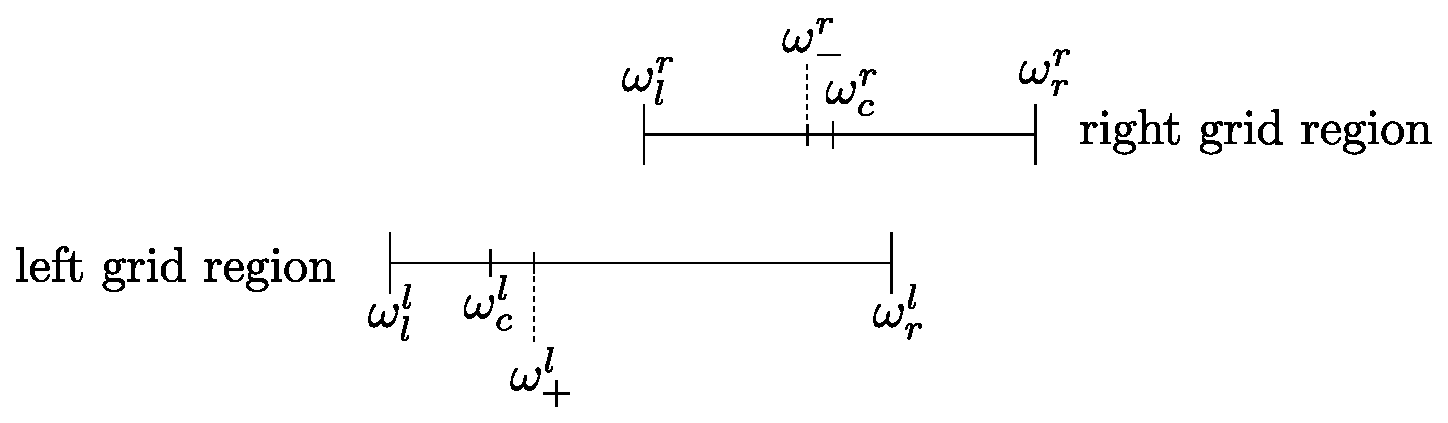
\includegraphics[width=0.8\textwidth]{pics/cutting_gr.eps}
	\caption{Nomenclature for the cutting of two intersecting grid regions}
	\label{fig:cutting_gr}
\end{figure}

The cutting point must be right from the center point of the left grid region plus a small grid dependent buffer, this point is called $\omega_+^l$ (see \ref{sec:grid_regions}). It also has to be left from the center point of the right grid region minus a small grid dependent buffer, this point is called $\omega_-^r$ (see \ref{sec:grid_regions}). Moreover the cutting point must not exceed the right boundary of the left grid region $\omega_r^l$ while at the same time it must not fall below the left boundary of the right grid region $\omega_l^r$. Therefore the cutting point $\omega_s$ must lie inside the following interval
\begin{equation}\label{eqn:cutting_point_boundaries}
	\omega_s \in [\,max(\omega_+^l, \omega_l^r)\,,\;\; min(\omega_-^r, \omega_r^l)\,]\;:=I
\end{equation}
In this intervall, the grid point density of the left grid region $\frac{di}{d\omega}|_l$ is monotonically decreasing and the grid point density of the right grid region $\frac{di}{d\omega}|_r$ is a monotonically increasing. The cutting point should be that point, where the grid point densities of both grid regions become equal
\begin{equation}\label{eqn:cutting_point}
	\left. \frac{di}{d\omega}\right|_l(\omega_s) \stackrel{!}{=} \left. \frac{di}{d\omega}\right|_r(\omega_s)
\end{equation}
This equation, can be solved analytically for all combinations of equidistant, tangential and logarithmic grid regions. This is done in appendix \ref{chapter:app_cutting_points}. The calculated cutting point does not always lie inside the interval $I$. In such a case one has to put more thought in what to do. This is done in the following where we list all possibilities which can occur if a solution to equation \ref{eqn:cutting_point} exists.

\begin{itemize} % itemize because cases label should be in agreement with source code
	\item{\bf Case A}: $\omega_s \in I$: If the calculated cutting point lies inside the interval $I$, both grids are cutted at this particular point so that there is no more intersection between the grids.

	\item{\bf Case B}: $\omega_s \notin I$ and $\omega_l^r \leq \omega_s < \omega_+^l$: This means, that the maximal resolution of the left grid is smaller than the resolution of the right grid at $\omega_+^l$. Therefore the purpose of the left grid region is assumed to be fullfilled, and it is skipped.
\end{itemize}
Of course there are cases, in which this point does not exists. For example, if the lowest resolution of one grid region is higher than the highest resolution of the other. 


\section{Subgrid and inserting grid regions}\label{sec:subgrids_and_insert}
\index{Subgrid}
\index{Inverse of the multigrid}
If all fundamental grid regions have gone through the cutting procedure explained in \ref{sec:cutting_procedure}, we are left with a bunch of non-intersection grid regions. These grid regions are now ready to be inserted into the basic grid region. But there is one difficulty we have not mentioned so far which is the fact that one has to take care of the inverse. Since all grid regions consist of one of the simple grid classes from chapter \ref{chapter:simple_grids}, their inverse mapping is know. 

\section{Inverse of the multigrid}\label{sec:inverse_of_the_multigrid}
\index{Inverse of the multigrid}



